% ---- Modele TP PC V2 -----------
\documentclass[a4paper,10pt,french]{scrartcl}
\usepackage[T1]{fontenc}%---pour l'encodage d'entr\'ee
\usepackage{array}%---pour les tableaux
\usepackage{titlesec}%---modification des titres
\usepackage{ulem}%---pour le soulignage
\usepackage[dvipsnames]{xcolor}%---pour avoir d'autres couleurs
\usepackage{color}%---pour avoir les couleurs de base
\usepackage{babel}%---pour les trucs de langue et la francisation

\usepackage{graphicx}%----pour mettre des images
\usepackage[utf8]{inputenc}%---encodage
\usepackage{geometry}%---pour modifier les tailles et mettre a4paper
%\usepackage{awesomebox}%---pour les boites d'exercices, de pbq et de croquis ---d\'esactiv\'e pour les TP de PC
\usepackage{tikz}%---pour dessiner + d\'ependance de chemfig
%\usepackage{tabularx}%---pour dimensionner automatiquement les tableaux avec variable X
\usepackage{fancyhdr}%---pour les en-t\^ete personnalis\'ees
\usepackage{blindtext}%---pour les liens
\usepackage{hyperref}%---pour les liens (\`a mettre en dernier)
\usepackage{caption}%---pour la francisation de la l\'egende table vers Tableau
 \usepackage{float}% --- pour placer les figures et tableaux où l'on souhaite avec argument H
 \usepackage{multicol}
 \usepackage{amsmath}
 \usepackage{geometry}
 \geometry{vmargin=2.5cm}

\captionsetup{labelfont=sc}%---pour la francisation de la l\'egende table vers Tableau
\def\frenchtablename{Tableau}%---pour la francisation de la l\'egende table vers Tableau
\pagestyle{fancy}
\renewcommand\headrulewidth{1pt}
\fancyhead[L]{TP 1}
\fancyhead[R]{Saux Paulhenry}
\title{Compte rendu de TP 6}
\date{}
\author{}

\geometry{a4paper}
% ----------- Création des commandes de couleur ----------
\makeatletter
\newcommand{\coloruline}[2]{%
        \UL@protected\def\temp@uline{\leavevmode \bgroup
            \markoverwith{\textcolor{#1}{\rule[-0.5ex]{2pt}{0.4pt}}}%
        \ULon}%
        \temp@uline{#2}%
    }

    \newcommand{\coloruuline}[2]{%
        \UL@protected\def\temp@uuline{\leavevmode \bgroup
            \UL@setULdepth
            \ifx\UL@on\UL@onin \advance\ULdepth2.8\p@\fi
            \markoverwith{\textcolor{#1}{\lower\ULdepth\hbox
                {\kern-.03em\vbox{\hrule width.2em\kern1\p@\hrule}\kern-.03em}}}%
        \ULon}%
        \temp@uuline{#2}%
    }

\makeatother

\renewcommand{\thesection}{\arabic{section}}
\renewcommand{\thesubsection}{\arabic{subsection}}
\renewcommand{\thesubsubsection}{\arabic{subsubsection}}
\begin{document}
% ---------------- Modification des titres de niveau 1,2 et 3 --------------------
\titleformat
{\section} % command
%[display] % shape
{\Large} % format
{\coloruuline{red}{\thesection. }} % label
{0ex} % sep
{\coloruuline{red}} % before-code
[] % after-code

\titleformat
{\paragraph} % command
%[display] % shape
{\Large} % format
{\coloruline{NavyBlue}{\theparagraph. }} % label
{0ex} % sep
{\coloruline{NavyBlue}} % before-code
[] % after-code

\titleformat
{\subsection} % command
%[display] % shape
{\Large} % format
{\coloruline{red}{\thesection.\thesubsection. }} % label
{0ex} % sep
{\coloruline{red}} % before-code
[] % after-code

\titleformat
{\subsubsection} % command
%[display] % shape
{\large} % format
{\coloruline{ForestGreen}{\thesection.\thesubsection.\thesubsubsection. }} % label
{0ex} % sep
{\coloruline{ForestGreen}} % before-code
[] % after-code

\titleformat
{\chapter} % command
%[display] % shape
{\large} % format
{\coloruline{NavyBlue}{\thechapter \:- }} % label
{0ex} % sep
{\coloruline{NavyBlue}} % before-code
[] % after-code


% ---------------- Début du corps du document ------------------------------------

\section{Introduction}
\subsection{Objectifs}
L'objectif de ce TP est de mettre en évidence les phénomènes de diffraction et d'interférences en lumière monochromatique à l'aide de divers instruments optiques. On se servira également des observations pour détermier certaines propriétés des instruments.
\subsection{Sommaire}
Ce TP se décompose en 5
parties :
\begin{enumerate}
 \item Observation de la diffraction
 \item Observation des interférences et détermination des propriétés du prisme
 \item Analyse des sources virtuelles crées par le prisme et détermination des propriétés du prisme
 \item Observation d'interférences et de la diffraction
 \item Analyse qualitative de bifentes
\end{enumerate}
\section{Protocole}
\subsection{Matériel}
\begin{itemize}
\item Photodiode
\item Voltmètre
\item Lentilles de focale 0.5m et 0.2m
\item Objectif de microscope
\item Prisme
\item Fente diffractante réglable
\item Rail optique
\item Supports pour rail optique
\item Supports à déplacement transversal pour rail optique
\item Laser
\item Écran
\end{itemize}
\subsection{Observation de la diffraction}
\subsubsection{Description du montage expérimental}
On place après le faisceau laser (1) la fente diffractante (2), la lentille de focale 0.5m (3), puis la photodiode (4) placée sur un pied à déplacement transversal, sur le foyer image de la lentille. La photodiode est connectée est Voltmètre. L'ensemble est aligné verticalement.
\begin{center}

\includegraphics[scale=0.7]{schema1}
\end{center}
\subsubsection{Mesures à effectuer}
\begin{itemize}
\item Éteindre le faisceau lumineux. Relever la valeur de tension de la photodiode
 \item Placer la bague de déplacement horizontal de la photodiode à 0. Relever la valeur de tension.
 \item Ajouter 2.00
 mm de déplacement horizontal et relever la tension
 \item Refaire l'étape précédente jusqu'à ce que la course du pied nous limite
 \item Autour de la position ou la photodiode est centrée horizontalement avec le montage, chercher la valeur de tension la plus haute et relever la valeur de déplacement
 \item Autour de cette position, cherche la valeur de déplacement pour laquelle la tension atteint son premier minium (avant et après le pic)
\end{itemize}
\subsection{Observation des interférences}
\subsubsection{Description du montage expérimental}
On place après le faisceau laser (1) un objectif de microscope (2), puis le prisme (3) à une distance l de cet objectif. L'objectif sera positionné à une distance de 2m de l'écran d'Observation.
\begin{center}

\includegraphics[scale=0.7]{schema2}
\end{center}
\subsubsection{Mesures à effectuer}
\begin{itemize}
\item Réaliser le montage expérimental
\item Mesurer sur l'écran à l'aide du papier millimétré la distance entre une dizaine de frange d'intéférence et relever le nombre exact de frange compris dans la mesure.
\end{itemize}
\subsection{Analyse des sources virtuelles crées par le prisme et détermination des propriétés du prisme}
\subsubsection{Description du montage expérimental}
On rajoute au montage précédent une lentille (4) L de focale 0.2m
\subsubsection{Mesures à effectuer}
\begin{itemize}
\item Réaliser le montage expérimental
\item Déplacer la lentille de façon à former sur l'écran l'image nette des 2 sources virtuelles
\item Mesurer la distance entre les 2 points projetés sur l'écran
\item Mesurer la distance SL et LE
\end{itemize}
\section{Mesures}
\subsection{Étude qualitative de la diffraction}
\begin{center}
\begin{tabular}{llll}
Conditions & Intensité & Largeur des taches & Direction de l'étalement\\
diminution de la largeur & Diminution & Augmentation & Inchangée\\
Rotation dans le plan & Inchangée & Inchangée & Perpendiculaire à la fente\\
Diminution de la distance D & Inchangée & Diminution & Inchangée
\end{tabular}
\end{center}

\subsection{Observations de la diffraction}
\subsubsection{Données}
\begin{table}[H]
\begin{center}
\begin{tabular}{ll}
x (mm) & U (mV)\\
0,00 & 20,0\\
2,00 & 23,9\\
4,00 & 18,5\\
6,00 & 26,2\\
8,00 & 25,4\\
10,00 & 41,6\\
10,65 & 20,0\\
12,00 & 25,3\\
14,00 & 539\\
14,6 & 561\\
16,00 & 380\\
18,00 & 28,0\\
18,2 & 20,0\\
20,00 & 41,0\\
22,00 & 20,0\\
24,00 & 23,0\\
25,00 & 19,7
\end{tabular}
\end{center}
\caption{Tensions mesurées en fonction du déplacement transversal}
\end{table}
\subsubsection{Incertitudes}
L'incertitude liée à la position transversale de la photodiode est liée à la précision de la vis de déplacement, de l'ordre de \(\frac{0.01}{\sqrt{3}}\)mm et celle sur la tension est liée uniquement la précision de l'appareil de mesure.

Cependant, elle est négligeable devant l'erreur systématique effectuée lors de la mesure de la tension. En effet, lorsque la photodiode n'est pas éclairée par le laser, la valeur de tension renvoyée n'est pas nulle. Elle est d'environ 20 mV.

De plus, la photodiode renvoie des valeurs de tension pour un intervalle de l'ordre de 1mm (taille de la fente de la Photodiode). Cette incertitude est à rajouter sur la position de x, donc \(u(x) = \pm 1\)mm.
\subsection{Observation des interférences}
\subsubsection{Données}
\begin{center}
\begin{tabular}{llll}
Nombre de franges & Distance mesurée sur l'écran (cm) & D (cm) & l (cm)\\
11 & 1.75 & 174.5 & 5.45
\end{tabular}
\end{center}
\subsubsection{Incertitude}
L'incertitude sur le nombre de frange est nulle. Celle sur la distance mesurée sur l'écran est liée à la précision de l'appareil de mesure, ici une règle ou papier gradué au mm près mais aussi à la capacité à placer correctement l'appareil de mesure sur l'écran de façon à faire une mesure précise (1mm). Il faut également ajouter l'incertitude liée à la largeur des franges (de l'ordre du mm). On estime donc l'incertitude liée la distance mesurée d'environ \(2\)mm. Pour trouver u(i), il faut la diviser par le nombre de franges mesurées.

La distance D est la différence de position de l'écran et de la source. Celle sur la position de l'écran sera considérée comme nulle (l'écran est à l'origine du rail et complètement collé). Celle sur la position de la source S est liée à la position de l'objectif mais aussi à sa distance focale, qui nous est inconnue.

L'incertitude liée à la position de l'objectif est produite par la graduation du rail et celle sur la focale est d'environ 2mm. On estime donc \(u(D) = 2mm\).

L'incertitude liée à l est aussi liée à la position de S, mais il faut rajouter l'incertitude liée à la position du prisme. Or, ce dernier n'est pas exactement centré sur le support, (décalage de 1mm), donc \(u(l) = u(S) + u(P) =  3mm\).
\subsection{Analyse des sources virtuelles}
\subsubsection{Données}
\begin{center}
\begin{tabular}{lllll}
Taille de l'image réelle (cm) & D (cm) & l (cm) & EL (cm) & LP (cm)\\
0.45 & 174.55 & 5.45 & 150.8 & 23.8
\end{tabular}
\end{center}
\subsubsection{Incertitude}
Les incertitudes sur D et L sont les m\^emes qu'en partie précédente. Celle sur EL est liée uniquement à la position de la lentille (l'écran est toujours à l'origine), soit \(\frac{0.1}{\sqrt{3}}\)cm et celle sur LS est principalement liée à la position de S dont on a déjà discuté. Donc \(u(LS) = 2\)mm.

L'incertitude sur la taille de l'image est liée à la précision de l'appareil de mesure mais aussi à la difficulté à la mesurer correctement. En effet, les 2 taches ont une largeur d'environ 1mm. On estimera donc l'incertitude à 2mm.
\subsection{Lien entre sources virtuelles et interfrange}
\begin{center}
\begin{tabular}{lll}
Taille de l'image réelle (cm) & D (cm) & l (cm)\\
0.75 & 174.55 & 5.45 \\
1.0 & 174.55 & 5.45
\end{tabular}
\end{center}
Les incertitudes sont les m\^emes qu'en partie précédente.
\subsection{Analyse qualitative de Bifentes}
\begin{center}
\begin{tabular}{lll}
Bifente & Interfrange de diffraction (cm) & Interfrange d'interférences (cm)\\
C & 1.0& 0.1\\
B & 2.3 & 0.23
\end{tabular}
\end{center}
Il s'agit d'une étude qualitative grossière, donc les incertitudes n'ont pas d'importance ici.
\section{Graphiques}
\subsection{Observation de la diffraction}
\begin{figure}[H]
 \begin{center}
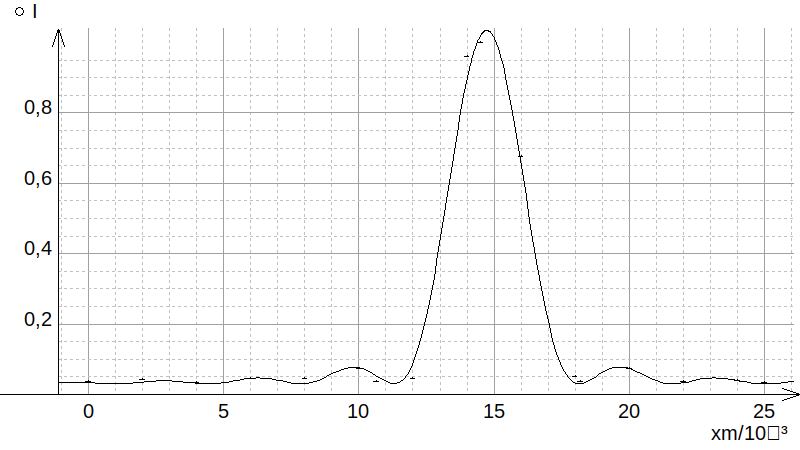
\includegraphics[scale=0.4]{tp1}
 \end{center}
\caption{Intensité mesurée en fonction du déplacement transversal (m)}
\end{figure}

\section{Exploitation des résultats}
\subsection{Étude qualitative de la diffraction}
\subsubsection{Diminution de la largeur de la fente (a)}
Les résultats sont cohérents avec la prédiction théorique.
L'intensité lumineuse totale qui traverse la fente est proportionnelle à la surface de la fente. Si la largeur $a$ diminue, la quantité de lumière qui passe est réduite, ce qui entraîne une diminution de l'intensité  observée. De plus, la largeur des taches L sont inversement proportionnels à la largeur de la fente $a$. Si a diminue, la largeur des taches sur l'écran augmentent. Ainsi, plus l'obstacle est petit, plus la diffraction est importante. Enfin, la direction de l'étalement est toujours perpendiculaire à l'axe long de la fente. La diminution de la largeur ne change donc pas l'orientation de cet axe.
\subsubsection{Rotation de la fente dans le plan}
La figure de diffraction s'étale toujours perpendiculairement à la fente (parallèlement à sa largeur). Si la fente tourne, l'orientation de la figure de diffraction tourne avec elle.
\subsubsection{Diminution de la distance de l'écran (D)}
La largeur L est directement proportionnelle à la distance D . Si la distance D entre la fente et l'écran diminue, la largeur L de la tache centrale diminue en proportion
\subsection{Observations de la diffraction}

On peut modéliser nos mesure par \[I=A\cdot\Big(\frac{\sin(\pi\cdot(x-x_0)/B)}{(\pi\cdot(x-x_0)/B)}\Big)^2+C\] avec \(I\propto \frac{U}{U_{max}}\). Les constantes A, B, \(x_0\) et C sont donnés par la regression linéaire. Le coefficient C est ajouté en raison de l'erreur systématique de la photodiode et \(x_0\) représente l'emplacement du maximum d'intensité. De cette façon, on obtient \(A=(1,027 \pm 0,020) SI, x_0=(14,728 \pm0,037)10^{-3} SI, B=(3,43 \pm0,11)10^{-3} SI, C=(30,5 \pm6,4)10^{-3} SI \).

On remarque que la valeur de \(x_0\) obtenue à partir de la régression correspond  à la valeur obtenue expérimentalement\footnote{Dans les données, c'est pour une valeur proche de $x_0$ que l'on obtient la tension la plus forte}, ce signifie que la modélisation semble fonctionner.

On peut déduire du coefficient B la valeur de la largeur de la fente utilisée. En effet, on sait que \[B = \frac{\lambda f'_1}{a} \] avec \(\lambda\) la longueur d'onde du laser et \(\lambda_1'\) la distance focale de la lentille utilisée. On déduit de cette relation, avec \(\lambda=632.8\cdot 10^{-9}SI, f'_1=0.5SI\) la largeur \(a = (9.22\cdot 10^{-5})\)SI.
\subsection{Observations des interférences}
On calcule l'interfrange avec \begin{equation}
                               i = \frac{d}{N}
                              \end{equation}
On trouve \(i = 0.1590 cm\).
On peut déduire de l'interfrange mesuré l'angle \(\theta\) du prisme utilisé.

En effet, on sait que \begin{equation}
                       i = \frac{\lambda D}{a}
                      \end{equation} avec D la Distance entre la source et l'écran et a la distance entre les 2 sources à l'origine des interférence, ici la distance entre les 2 sources virtuelles du prisme.

De plus, dans l'approximation des petits angles, on a une relation entre \(l\), la distance entre la source et le prisme, \(a\), la distance entre les 2 sources virtuelles et \(\theta\), l'angle du prisme :

\[\theta = \frac{a}{2l}\]

Dès lors, on a la relation \begin{equation}
                            \theta = \frac{\lambda D}{2il}
                           \end{equation}

et \[u(\theta) = \theta \times \sqrt{(\frac{u(D)}{D})^2 + ()\frac{u(i)}{i})^2 + (\frac{u(l)}{l})^2} \]
Les incertitudes relatives sont :
\begin{itemize}
    \item $\frac{u(D)}{D} = \frac{0.2}{174.5} \approx 0.00115$
    \item $\frac{u(i)}{i} = \frac{0.0182}{0.1590} \approx 0.1145$
    \item $\frac{u(l)}{l} = \frac{0.3}{5.45} \approx 0.0550$
\end{itemize}
Ainsi, $\frac{u(\theta)}{\theta} \approx \sqrt{0.00115^2 + 0.1145^2 + 0.0550^2} \approx \sqrt{0.01608} \approx 0.1268$.
Avec $\theta = 6.39\cdot 10^{-3}\text{ rad}$, l'incertitude absolue est $u(\theta) \approx (6.39\cdot 10^{-3}) \times 0.1268 \approx 0.81\cdot 10^{-3}\text{ rad}$.
On trouve alors $\theta = (6.39 \pm 0.81)\cdot 10^{-3}\text{ rad}$.


\subsection{Analyse des sources virtuelles}
Cette partie va nous servir à confirmer l'angle \(\theta\) du prisme trouvé en partie précédente. Pour ce faire, on déterminera la distance entre les 2 sources virtuelles non pas par l'optique ondulatoire mais par des considérations d'optique géométriques.

On sait que le grandissement est donné par \begin{equation}
                                            \gamma = \frac{EL}{LP} = \frac{a'}{a}
                                           \end{equation} avec \(a'\) la taille de l'image réelle des 2 sources virtuelles.
Connaissant 3 des quatre inconnues, on peut déterminer \(a\). On aura alors \begin{equation}
                                                                             \theta = \frac{a'LP}{EL2l}
                                                                            \end{equation}
et \[u(\theta) = \theta \times \sqrt{(\frac{u(EL)}{EL})^2 + ()\frac{u(LP)}{LP})^2 + (\frac{u(l)}{l})^2} \]
Les incertitudes relatives sont :
\begin{itemize}
    \item $\frac{u(a')}{a'} = \frac{0.2}{0.45} \approx 0.4444$
    \item $\frac{u(LP)}{LP} = \frac{0.2}{23.8} \approx 0.00840$
    \item $\frac{u(EL)}{EL} = \frac{0.1/\sqrt{3}}{150.8} \approx 0.000383$
    \item $\frac{u(l)}{l} = \frac{0.3}{5.45} \approx 0.0550$
\end{itemize}
Ainsi, $\frac{u(\theta)}{\theta} \approx \sqrt{0.4444^2 + 0.00840^2 + 0.000383^2 + 0.0550^2} \approx \sqrt{0.2006} \approx 0.4479$.
Avec $\theta = 6.46\cdot 10^{-3}\text{ rad}$, l'incertitude absolue est $u(\theta) \approx (6.46\cdot 10^{-3}) \times 0.4479 \approx 2.89\cdot 10^{-3}\text{ rad}$.
On trouve alors $\theta = (6.46 \pm 2.89)\cdot 10^{-3}\text{ rad}$.
\subsection{Lien entre sources virtuelles et interfrange}
Les résultats sont cohérents avec les prédictions théoriques. En effet, quand \(l\) augmente, \(a\) augmente, car \(\theta = \frac{a}{2l}\) et donc \(i\) diminue car inversement proportionnel à a. Comme \(a'\propto a\) par \((4)\) (le grandissement est fixe car EL et LP sont fixes), le fait que \(a'\) augmente avec \(l\) montre bien que l'interfrange diminue (car \(a'\propto a \propto i^{-1}\)).
\subsection{Analyse des bifentes}
Le phénomène observé avec une bifente est une combinaison de deux effets : les interférences et la diffraction.

La bifente C a ses 2 fentes plus éloignées que la bifente B ($b_C > b_B$).

L'interfrange d'interférences est inversement proportionnel à l'écartement $b$ entre les fentes.
Pour la bifente C ($i_{\text{int}, C} = 0.1 \text{ cm}$), l'interfrange est plus petit que celui de la bifente B ($i_{\text{int}, B} = 0.23 \text{ cm}$).
Puisque $i_{\text{int}, C} < i_{\text{int}, B}$, cela implique $\mathbf{b_C > b_B}$.
Ceci est en parfaite cohérence avec l'hypothèse fournie, car plus les sources (fentes) sont éloignées, plus les franges d'interférences sont serrées.

L'interfrange de diffraction (qui représente la demi-largeur de l'enveloppe centrale $L_{\text{diff}}$) est inversement proportionnel à la largeur $a$ de chaque fente ($L_{\text{diff}} \propto 1/a$).
La bifente C présente une enveloppe de diffraction plus petite ($i_{\text{diff}, C} = 1.0 \text{ cm}$) que celle de la bifente B ($i_{\text{diff}, B} = 2.3 \text{ cm}$).Puisque $i_{\text{diff}, C} < i_{\text{diff}, B}$, cela implique que $\mathbf{a_C > a_B}$.
Cette observation suggère que la fente C est également plus large que la fente B. La fente la plus large produit l'enveloppe de diffraction la plus étroite.

\section{Conclusion}
L'objectif était de valider les modèles de l'optique ondulatoire (diffraction et interférences).

Les valeurs centrales obtenues par les deux méthodes sont très proches. L'écart relatif entre elles est calculé par :
$$ \text{Écart Relatif} = \left|\frac{\theta_{i} - \theta_{g}}{\frac{\theta_{i} + \theta_{g}}{2}}\right| \times 100 \% = \left|\frac{6.39 - 6.46}{6.425}\right| \times 100 \% \approx 1.09 \% $$
Cet écart très faible démontre une bonne cohérence entre les 2 méthodes de mesure. De plus, les intervalles d'incertitude se chevauchent, ce qui confirme la compatibilité des mesures.

L'analyse des incertitudes révèle que les contributions majeures proviennent des mesures directes de distances sur l'écran et la source, ainsi que sur l'image réelle des sources virtuelles. l'incertitude de l'interfrange i reste la principale source d'erreur dans la méthode ondulatoire. Il faudrait mesurer la distance sur un plus grand nombre de franges (et donc augmenter la luminosité pour en observer plus) ou utiliser une la photodiode pour déterminer les centres des franges avec meilleure une précision.
\end{document}
